\documentclass[a4paper,12pt]{article} % тип документа

% Поля страниц
\usepackage[left=2.5cm,right=2.5cm,
    top=2cm,bottom=2cm,bindingoffset=0cm]{geometry}
    
%Пакет дял таблиц   
\usepackage{multirow} 
    
%Отступ после заголовка    
\usepackage{indentfirst}


% Рисунки
\usepackage{floatrow,graphicx,calc}
\usepackage{wrapfig}

% Создаёем новый разделитель
\DeclareFloatSeparators{mysep}{\hspace{1cm}}

% Ссылки?
\usepackage{hyperref}
\usepackage[rgb]{xcolor}
\hypersetup{				% Гиперссылки
    colorlinks=true,       	% false: ссылки в рамках
	urlcolor=blue          % на URL
}


%  Русский язык
\usepackage[T2A]{fontenc}			% кодировка
\usepackage[utf8]{inputenc}			% кодировка исходного текста
\usepackage[english,russian]{babel}	% локализация и переносы


% Математика
\usepackage{amsmath,amsfonts,amssymb,amsthm,mathtools}


% Что-то 
\usepackage{wasysym}


\begin{document}
\begin{center}
	\footnotesize{ФЕДЕРАЛЬНОЕ ГОСУДАРСТВЕННОЕ АВТОНОМНОЕ ОБРАЗОВАТЕЛЬНОЕ 			УЧРЕЖДЕНИЕ ВЫСШЕГО ОБРАЗОВАНИЯ}\\
	\footnotesize{МОСКОВСКИЙ ФИЗИКО-ТЕХНИЧЕСКИЙ ИНСТИТУТ\\(НАЦИОНАЛЬНЫЙ 			ИССЛЕДОВАТЕЛЬСКИЙ УНИВЕРСИТЕТ)}\\
	\footnotesize{ФАКУЛЬТЕТ ОБЩЕЙ И ПРИКЛАДНОЙ ФИЗИКИ\\}
	\hfill \break
	\hfill\break
	\hfill\break
	\hfill \break
	\hfill \break
	\hfill \break
	\hfill \break
	\hfill \break
	\hfill \break
	\hfill \break
	\hfill \break
	\hfill \break
	\hfill \break
	\hfill \break
	\large{Лабораторная работа № 2.5.1\\\textbf{Измерение коэффициента поверхностного натяжения жидкости}}\\
	\hfill \break
	\hfill \break
	\hfill \break
	\begin{flushright}
		Серебренников Даниил\\
		Группа Б02-826
	\end{flushright}
	\hfill \break
	\hfill \break
	\hfill \break
	\hfill \break
	\hfill \break
\end{center}
\hfill \break
\hfill \break
\hfill \break
\hfill \break
\hfill \break
\hfill \break
\begin{center}
	Долгопрудный, 2019 г.
\end{center}
\thispagestyle{empty}
\newpage
	\textbf{Цель работы:} 1) измерение температурной зависимости  коэффициента поверхностного натяжения дистиллированной воды с использованием известного коэффициента поверхностного натяжения спирта; 2) определение полной поверхностной энергии  и теплоты, необходимой для изотермического образования единицы поверхности жидкости  при различной температуре.\\
	\textbf{В работе используются:} прибор  Ребиндера  с термостатом и микроманометром; исследуемые жидкости; стаканы.
\section{Теоретическая часть}
	Наличие поверхностного слоя приводит к различию давлений по разные стороны от искривленной границы раздела двух сред. Для сферического пузырька с воздухом  внутри жидкости избыточное давление даётся формулой Лапласа:
	\begin{equation}
		\label{laplas}
		\Delta P = \frac{2\sigma}{r},
	\end{equation}
	где $\sigma$ – коэффициент поверхностного натяжения, $\Delta P$ – разница давлений внутри и снаружи пузырька, $r$ – радиус кривизны поверхности раздела двух фаз. Эта формула лежит в основе предлагаемого метода определения коэффициента поверхностного натяжения жидкости.
\section{Экспериментальная установка}
	Исследуемая жидкость (дистиллированная вода) наливается в сосуд (колбу) \textbf{В} (рис.~\ref{ris:ustanovka}). Тестовая жидкость  (этиловый спирт) наливается  в сосуд \textbf{E}. При измерениях  колбы герметично закрываются  пробками.   Через одну из двух пробок  проходит полая металлическая игла \textbf{C}. Этой пробкой закрывается сосуд, в котором  проводятся измерения. Верхний конец иглы открыт в атмосферу, а нижний погружен в жидкость. Другой сосуд герметично закрывается второй пробкой. При создании достаточного  разряжения воздуха в колбе с иглой пузырьки воздуха начинают пробулькивать через жидкость. Поверхностное натяжение можно определить по величине разряжения $\Delta P$ (\ref{laplas}), необходимого для прохождения пузырьков (при известном радиусе иглы).\\
	Разряжение в системе создается с помощью аспиратора \textbf{A}. Кран \textbf{K2} разделяет две полости аспиратора. Верхняя полость при закрытом кране \textbf{K2}  заполняется водой. Затем кран \textbf{K2} открывают и заполняют водой  нижнюю полость  аспиратора.  Разряжение воздуха создается в нижней полости  при открывании крана \textbf{K1}, когда  вода вытекает из неё по каплям. В колбах \textbf{B} и \textbf{C}, соединённых трубками с нижней полостью аспиратора,  создается такое же пониженное давление. Разность давлений в полостях с разряженным воздухом и атмосферой измеряется спиртовым микроманометром.
	\begin{figure}[H]
		\center{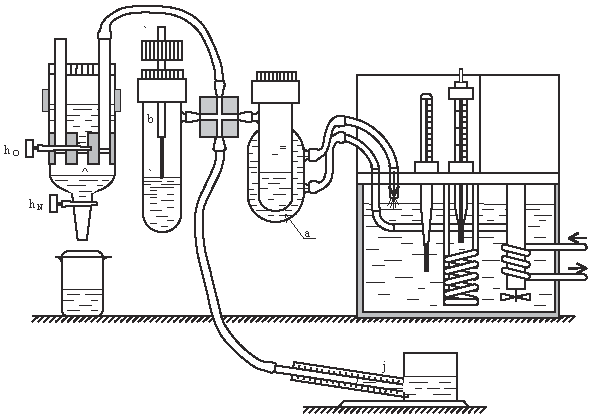
\includegraphics[scale=1]{Ustanovka.pdf}}
		\caption{Схема установки для измерения температурной зависимости коэффициента поверхностного натяжения.}
		\label{ris:ustanovka}
	\end{figure}
\section{Экспериментальные данные}
	В таблице~\ref{table:const} приведены константы, используемые в лабораторной работе. 	
\floatsetup[table]{capposition=top}	
\begin{table}[H]
	\caption{Постоянные величины.}
	\label{table:const}
\begin{tabular}{|c|c|c|c|c|}
	\hline
	\begin{tabular}[c]{@{}c@{}}Плотность\\ этанола\\ $\rho_0$, кг/м$^3$\end{tabular} & \begin{tabular}[c]{@{}c@{}}Плотность\\ воды\\ $\rho$, кг/м$^3$\end{tabular} & \begin{tabular}[c]{@{}c@{}}Ускорение\\ свободного падения\\ $g$, м/c$^2$\end{tabular} & \begin{tabular}[c]{@{}c@{}}Пересчетный\\ коэффициент\\ $k$\end{tabular} & \begin{tabular}[c]{@{}c@{}}Коэффициент\\ поверхностного натяжения\\ этанола (T = 20$^\circ$С)\\ $\sigma_0$, мН/м\end{tabular} \\ \hline
	809,5                                                                            & 1000,0                                                                      & 9,81                                                                                  & 0,2                                                                     & 22,75                                                                                                                         \\ \hline
\end{tabular}
\end{table}


	В таблице~\ref{table:error} приведены значения и случайные ошибки измерения величин, определяемых в ходе эксперимента.
\floatsetup[table]{capposition=top}	
\begin{table}[H]
	\caption{Некоторые величины и их погрешность.}
	\label{table:error}
\begin{tabular}{|c|c|c|c|}
	\hline
	& \begin{tabular}[c]{@{}c@{}}Температура\\ $T$, К\end{tabular} & \begin{tabular}[c]{@{}c@{}}Длина столба спирта\\ в микроманометре\\ $h$, мм\end{tabular} & \begin{tabular}[c]{@{}c@{}}Пересчитанные показания\\ микроманометра\\ $P$, Па\end{tabular} \\ \hline
	Величина          & 293,0                                                        & 175,0                                                                                      & 277,9                                                                                     \\ \hline
	Погрешность       & 0,1                                                          & 0,5                                                                                      & 0,8                                                                                       \\ \hline
	$\varepsilon$, \% & 0,03                                                         & 0,3                                                                                     & 0,3                                                                                       \\ \hline
\end{tabular}
\end{table}


	Результаты измерений радиуса иглы приведены в таблице~\ref{table:radius}. Для проверки достоверности полученного результата диаметр иглы был измерен дополнительно на микроскопе: $d = 1,34 мм$.
\floatsetup[table]{capposition=top}	
\begin{table}[H]
	\caption{Радиус используемой иглы.}
	\label{table:radius}
\begin{tabular}{|c|c|c|c|c|c|}
	\hline
	$T$, $^\circ$C & $h$, мм & $\Delta P$, Па & $r$, мм & $\sigma_r$, мм & $\sigma_r / r$, \% \\ \hline
	22,7           & 43    & 68,29          & 0,666   & 0,008          & 1,2                \\ \hline
\end{tabular}
\end{table}	


	В таблице~\ref{table:main} приведены результаты измерений\footnote{$\Delta P = \Delta \tilde{P} - \rho g \Delta h$, где $\Delta \tilde{P}$ -- давление, измеренное манометром; $\rho g \Delta h$ -- гидростатические давление воды ($\Delta h = 95$ мм).}, позволяющих исследовать зависимость $\sigma = \sigma (T)$.
\floatsetup[table]{capposition=top}	
\begin{table}[H]
	\caption{Результаты измерений.}
	\label{table:main}
\begin{tabular}{|c|c|c|c|c|c|}
	\hline
	$T$, $^\circ$C & $h$, мм & $\Delta P$, Па & $\sigma$, мН/м & $\sigma_\sigma$, мН/м & $\sigma_\sigma / \sigma$, \% \\ \hline
	23,0           & 181,0   & 194,3          & 65,1           & 0,8                   & 1,3                          \\ \hline
	25,6           & 179,0   & 191,1          & 64,0           & 0,8                   & 1,3                          \\ \hline
	30,5           & 180,0   & 192,7          & 64,6           & 0,8                   & 1,3                          \\ \hline
	35,3           & 177,0   & 187,9          & 63,0           & 0,8                   & 1,3                          \\ \hline
	40,1           & 176,6   & 187,3          & 62,7           & 0,8                   & 1,3                          \\ \hline
	45,0           & 175,0   & 184,7          & 62,0           & 0,8                   & 1,3                          \\ \hline
	50,0           & 172,6   & 180,9          & 60,6           & 0,8                   & 1,3                          \\ \hline
	55,0           & 172,0   & 180,0          & 60,3           & 0,8                   & 1,3                          \\ \hline
	60,0           & 171,0   & 178,4          & 59,8           & 0,8                   & 1,3                          \\ \hline
\end{tabular}
\end{table}


	По полученным данным построим график зависимости $\sigma = \sigma (T)$ (рис.~\ref{ris:Graph_1}) и проанализируем его (\ref{table:Graph_1}).
	\begin{figure}[H]
		\center{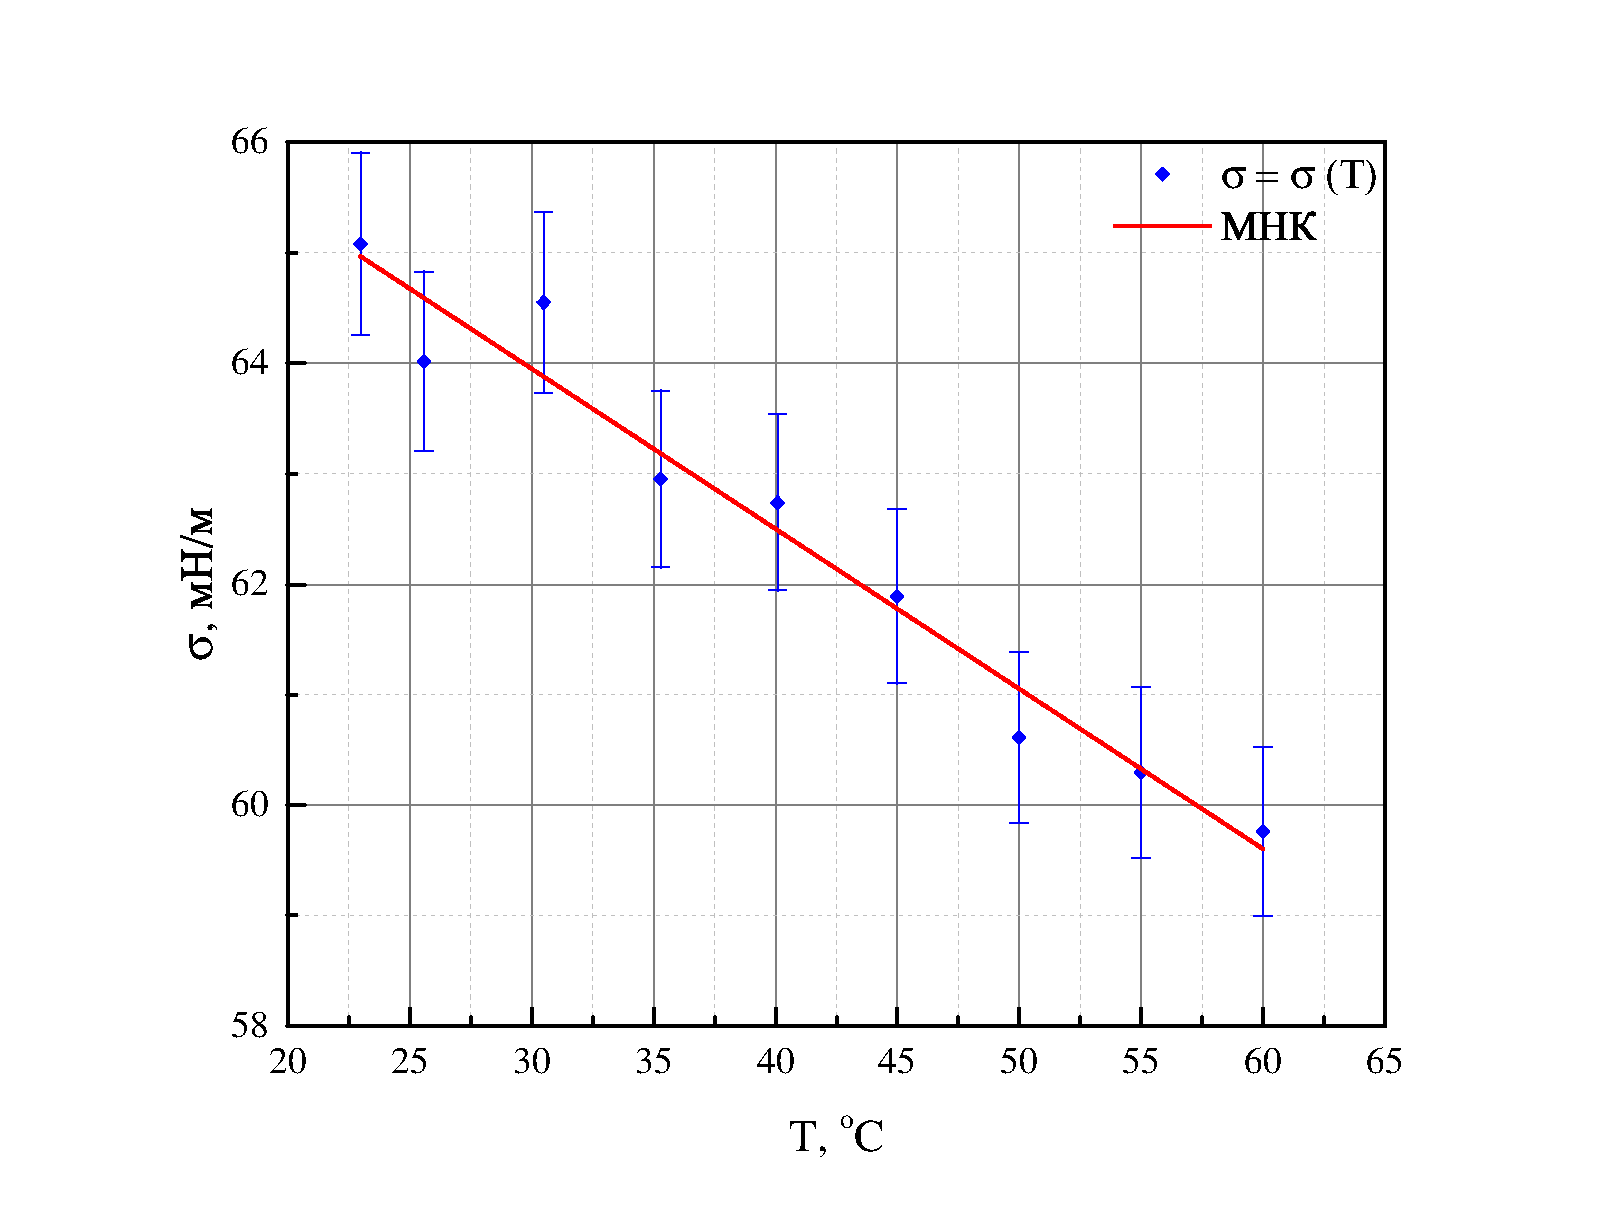
\includegraphics[scale=0.5]{Graph_1.pdf}}
		\caption{Зависимость $\sigma = \sigma (T)$.}
		\label{ris:Graph_1}
	\end{figure}


\floatsetup[table]{capposition=top}	
\begin{table}[H]
	\caption{Анализ зависимости $\sigma = \sigma (T)$.}
	\label{table:Graph_1}
\begin{tabular}{|c|c|c|}
	\hline
	$d\sigma / d T$, мН/м$\cdot^\circ$C & Погрешность, мН/м$\cdot^\circ$C & $\epsilon$, \% \\ \hline
	-0,15                               & 0,01                            & 6,7            \\ \hline
\end{tabular}
\end{table}


	Дополнительно найдем зависимость теплоты образования единицы поверхности жидкости $q =~-T\frac{d\sigma}{dT}$ и поверхностной энергии единицы площади $U/\Pi =~\sigma - q$ от температуры. Результаты вычислений представлены в таблице~\ref{table:Graph_2-3}, а графики на рис.~\ref{fig:Graph_2} и рис.~\ref{fig:Graph_3}.
	\floatsetup[table]{capposition=top}	
	\begin{table}[H]
		\caption{Результаты дополнительных вычислений.}
		\label{table:Graph_2-3}
\begin{tabular}{|c|c|c|c|c|c|c|c|c|c|}
\hline
$T$, К        & 296 & 298,6 & 303,5 & 308,3 & 313,1 & 318 & 323 & 328 & 333 \\ \hline
$q$, мДж/м$^2$     & 44  & 45    & 46    & 46    & 47    & 48  & 48  & 49  & 50  \\ \hline
$U/\Pi$, мДж/м$^2$ & 109 & 109   & 110   & 109   & 110   & 110 & 109 & 109 & 110 \\ \hline
\end{tabular}
	\end{table}
	
	
	\thisfloatsetup{floatrowsep=mysep}	
	\begin{figure}[h!]
		\begin{floatrow}
			\ffigbox[\FBwidth]{\caption{Зависимость $q = q(T)$.}\label{fig:Graph_2}}%
			{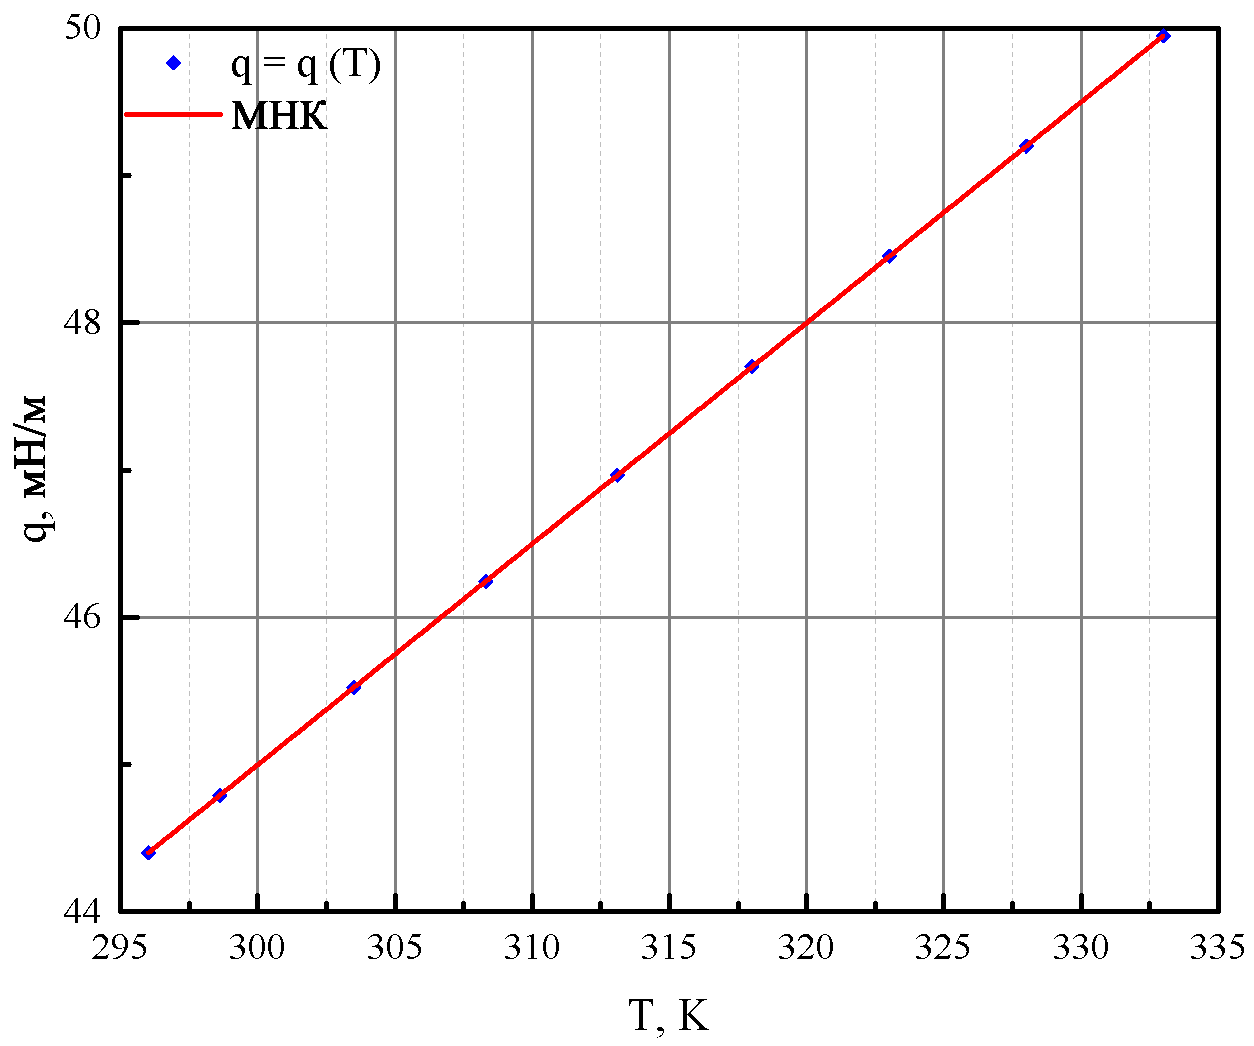
\includegraphics[width=8cm,height=7cm]{Graph_2}}
			\ffigbox[\FBwidth]{\caption{Зависимость $U/\Pi$ от $T$.}\label{fig:Graph_3}}%
			{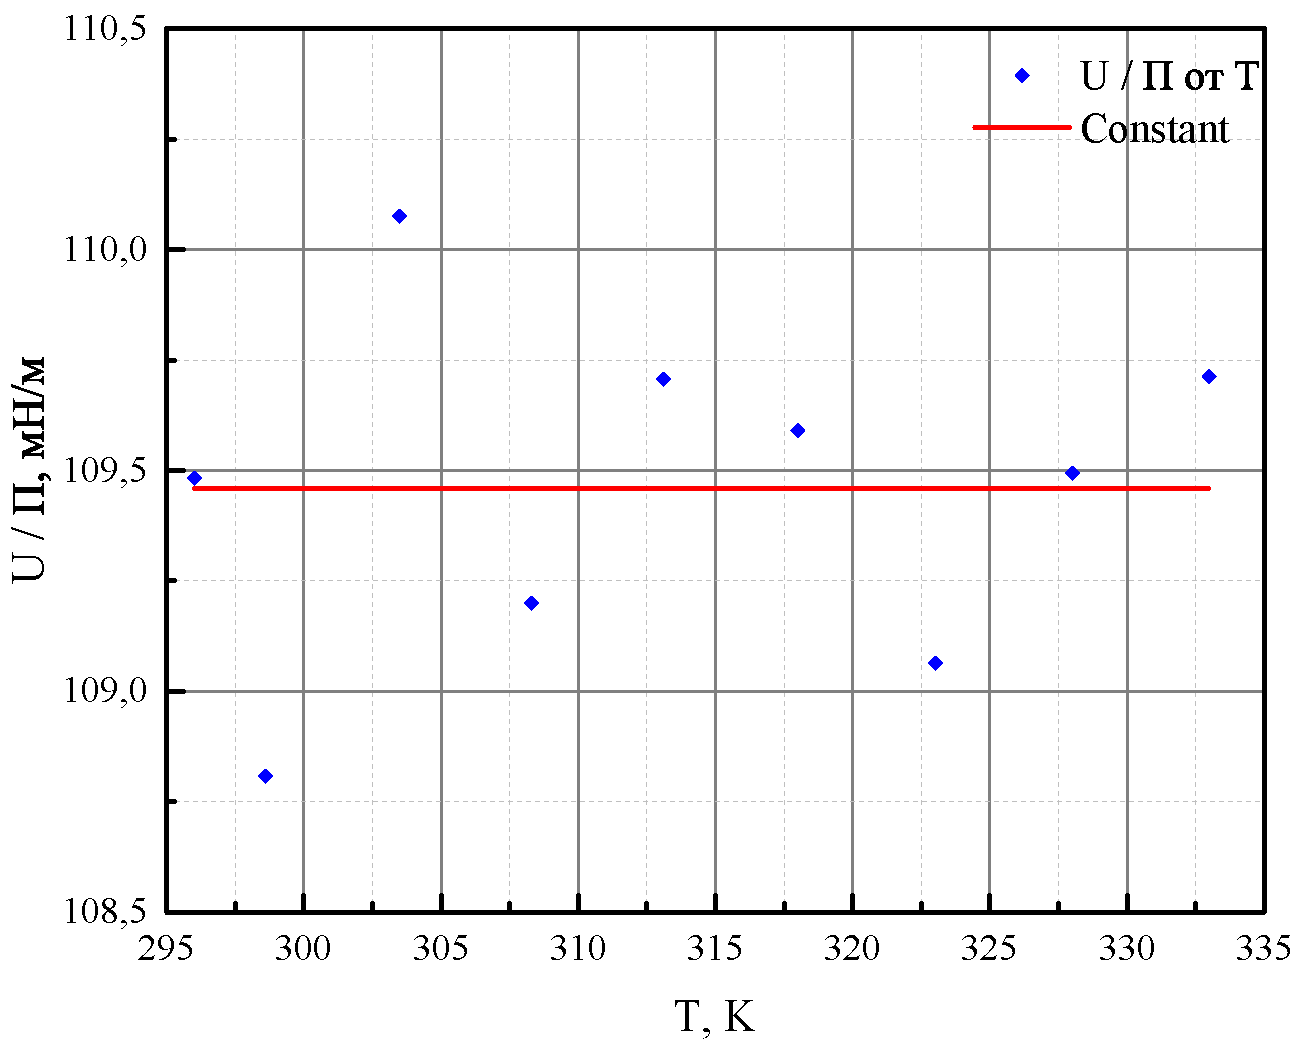
\includegraphics[width=8cm,height=7cm]{Graph_3}}         
		\end{floatrow}
	\end{figure}

\newpage
\section*{Обсуждение результатов}
	В ходе данной лабораторной работы мы исследовали температурную зависимость коэффициента поверхностного натяжения дистиллированной воды от температуры. Полученная зависимость оказалась линейной в интервале рабочих температур от 23$^\circ$C до 60$^\circ$C с коэффициентом наклона $d\sigma / dT = (-0,15\,\pm\, 0,01)$  мН/м$\cdot^\circ$C. Мы получили вполне естественный результат, потому что с увеличением температуры интенсивность межмолекулярного взаимодействия уменьшается, поэтому снижается и поверхностное натяжение жидкостей на границе с воздухом или с собственным паром. Вдали от критической температуры поверхностное натяжение уменьшается прямо пропорционально росту температуры. Стоит отметить, что наш результат в пределах погрешности совпадает с табличным значением $d\sigma / dT \approx -0,16$.
	
	Зная температурный коэффициент поверхностного натяжения, можно исследовать зависимость теплоты образования единицы поверхности жидкости $q = q(T)$ и поверхностной энергии единицы площади $U/\Pi$ от температуры. Если коэффициент поверхностного натяжения линейно зависит от температуры, то очевидно, что функция $q =-T\frac{d\sigma}{dT}$ является линейной. Менее тривиальным является вопрос о независимости внутренней энергии поверхности $U/\Pi$ от температуры. Для теоретического подтверждения экспериментального результата запишем уравнение Гиббса-Гельмгольца для поверхностного слоя $U/\Pi = \sigma - T\frac{d\sigma}{dT}$ и продифференцируем его по температуре: $\frac{\partial U/\Pi}{\partial T} = -T \frac{\partial^2 \sigma}{\partial T^2}$, но так как первая производная $\sigma$ по $T$ есть величина постоянная, то вторая производная обнуляется, следовательно, внутренняя энергия поверхностного слоя не зависит от температуры.
	
	
\section*{Выводы}
\begin{itemize}
	\item 
		В интервале температур от 23$^\circ$C до 60$^\circ$C зависимость $\sigma = \sigma(T)$ является линейной с коэффициентом наклона $d\sigma / dT = (-0,15\,\pm\, 0,01)$  мН/м$\cdot^\circ$C.
	\item 
		Теплоты образования единицы поверхности жидкости $q = q(T)$ линейно зависит от температуры вдали от критической точки.
	\item 	
		Внутренняя энергия поверхности $U/\Pi$ не зависит от температуры и есть константа $U = 109,5$ мДж/м$^2$.
\end{itemize}	
\end{document}